\documentclass{article}

\usepackage[letterpaper, portrait, margin=1.5in]{geometry}

\usepackage{fancyhdr}
\usepackage{ragged2e}
\usepackage{graphicx}
\usepackage{caption}
\usepackage{amsmath}
\usepackage{rotating}

\usepackage{listings}
\usepackage{color}

\definecolor{dkgreen}{rgb}{0,0.6,0}
\definecolor{gray}{rgb}{0.5,0.5,0.5}
\definecolor{mauve}{rgb}{0.58,0,0.82}

\lstset{frame=tb,
  language=Java,
  aboveskip=3mm,
  belowskip=3mm,
  showstringspaces=false,
  columns=flexible,
  basicstyle={\small\ttfamily},
  numbers=none,
  numberstyle=\tiny\color{gray},
  keywordstyle=\color{blue},
  commentstyle=\color{dkgreen},
  stringstyle=\color{mauve},
  breaklines=true,
  breakatwhitespace=true,
  tabsize=4
}

\setcounter{secnumdepth}{1}

\usepackage{chngcntr}
\counterwithin{figure}{section}

\renewcommand*{\thepage}{C\arabic{page}}

\pagestyle{fancy}
\lhead{ACME Robotics}
\chead{\#8367}
\rhead{\ifcontents Contents \else Week \thesection \fi}

\newif\ifcontents
\contentstrue

\makeatletter
\renewcommand{\@seccntformat}[1]{}
\makeatother
\begin{document}

\subsection{Diverter}
%!Prototyping an alternate sorting system.
After the Burlingame tournament the team realized how complicated their approach to sorting and depositing the minerals in the lander were. This was because the system had too many steps and required too many different parts and space. After the tournament, various members of the team started hypothesizing of alternative solutions to sorting. One solution that was thought up was a single cartridge for the balls and cubes to go into where they would be read by color sensors to determine the arrangement of balls or cubes. When dumped in the lander a diverter would be used to push the balls or cubes in the one direction or the other to allow for easily scoring ten points. Ashlin and Aidan took on the task of prototyping this diverter. A problem they noticed is that the if the combination of minerals had both a ball and a cube then both items would roll out so fast that the diverter wouldn't be fast enough to sort the minerals. They fixed this problem by implementing a gate that would separate the two minerals and cause a delay between them so the diverter would have time to re-position. Aidan and Kelly tested this the diverter and found it worked fairly accurately.

\begin{figure}
    \centering
    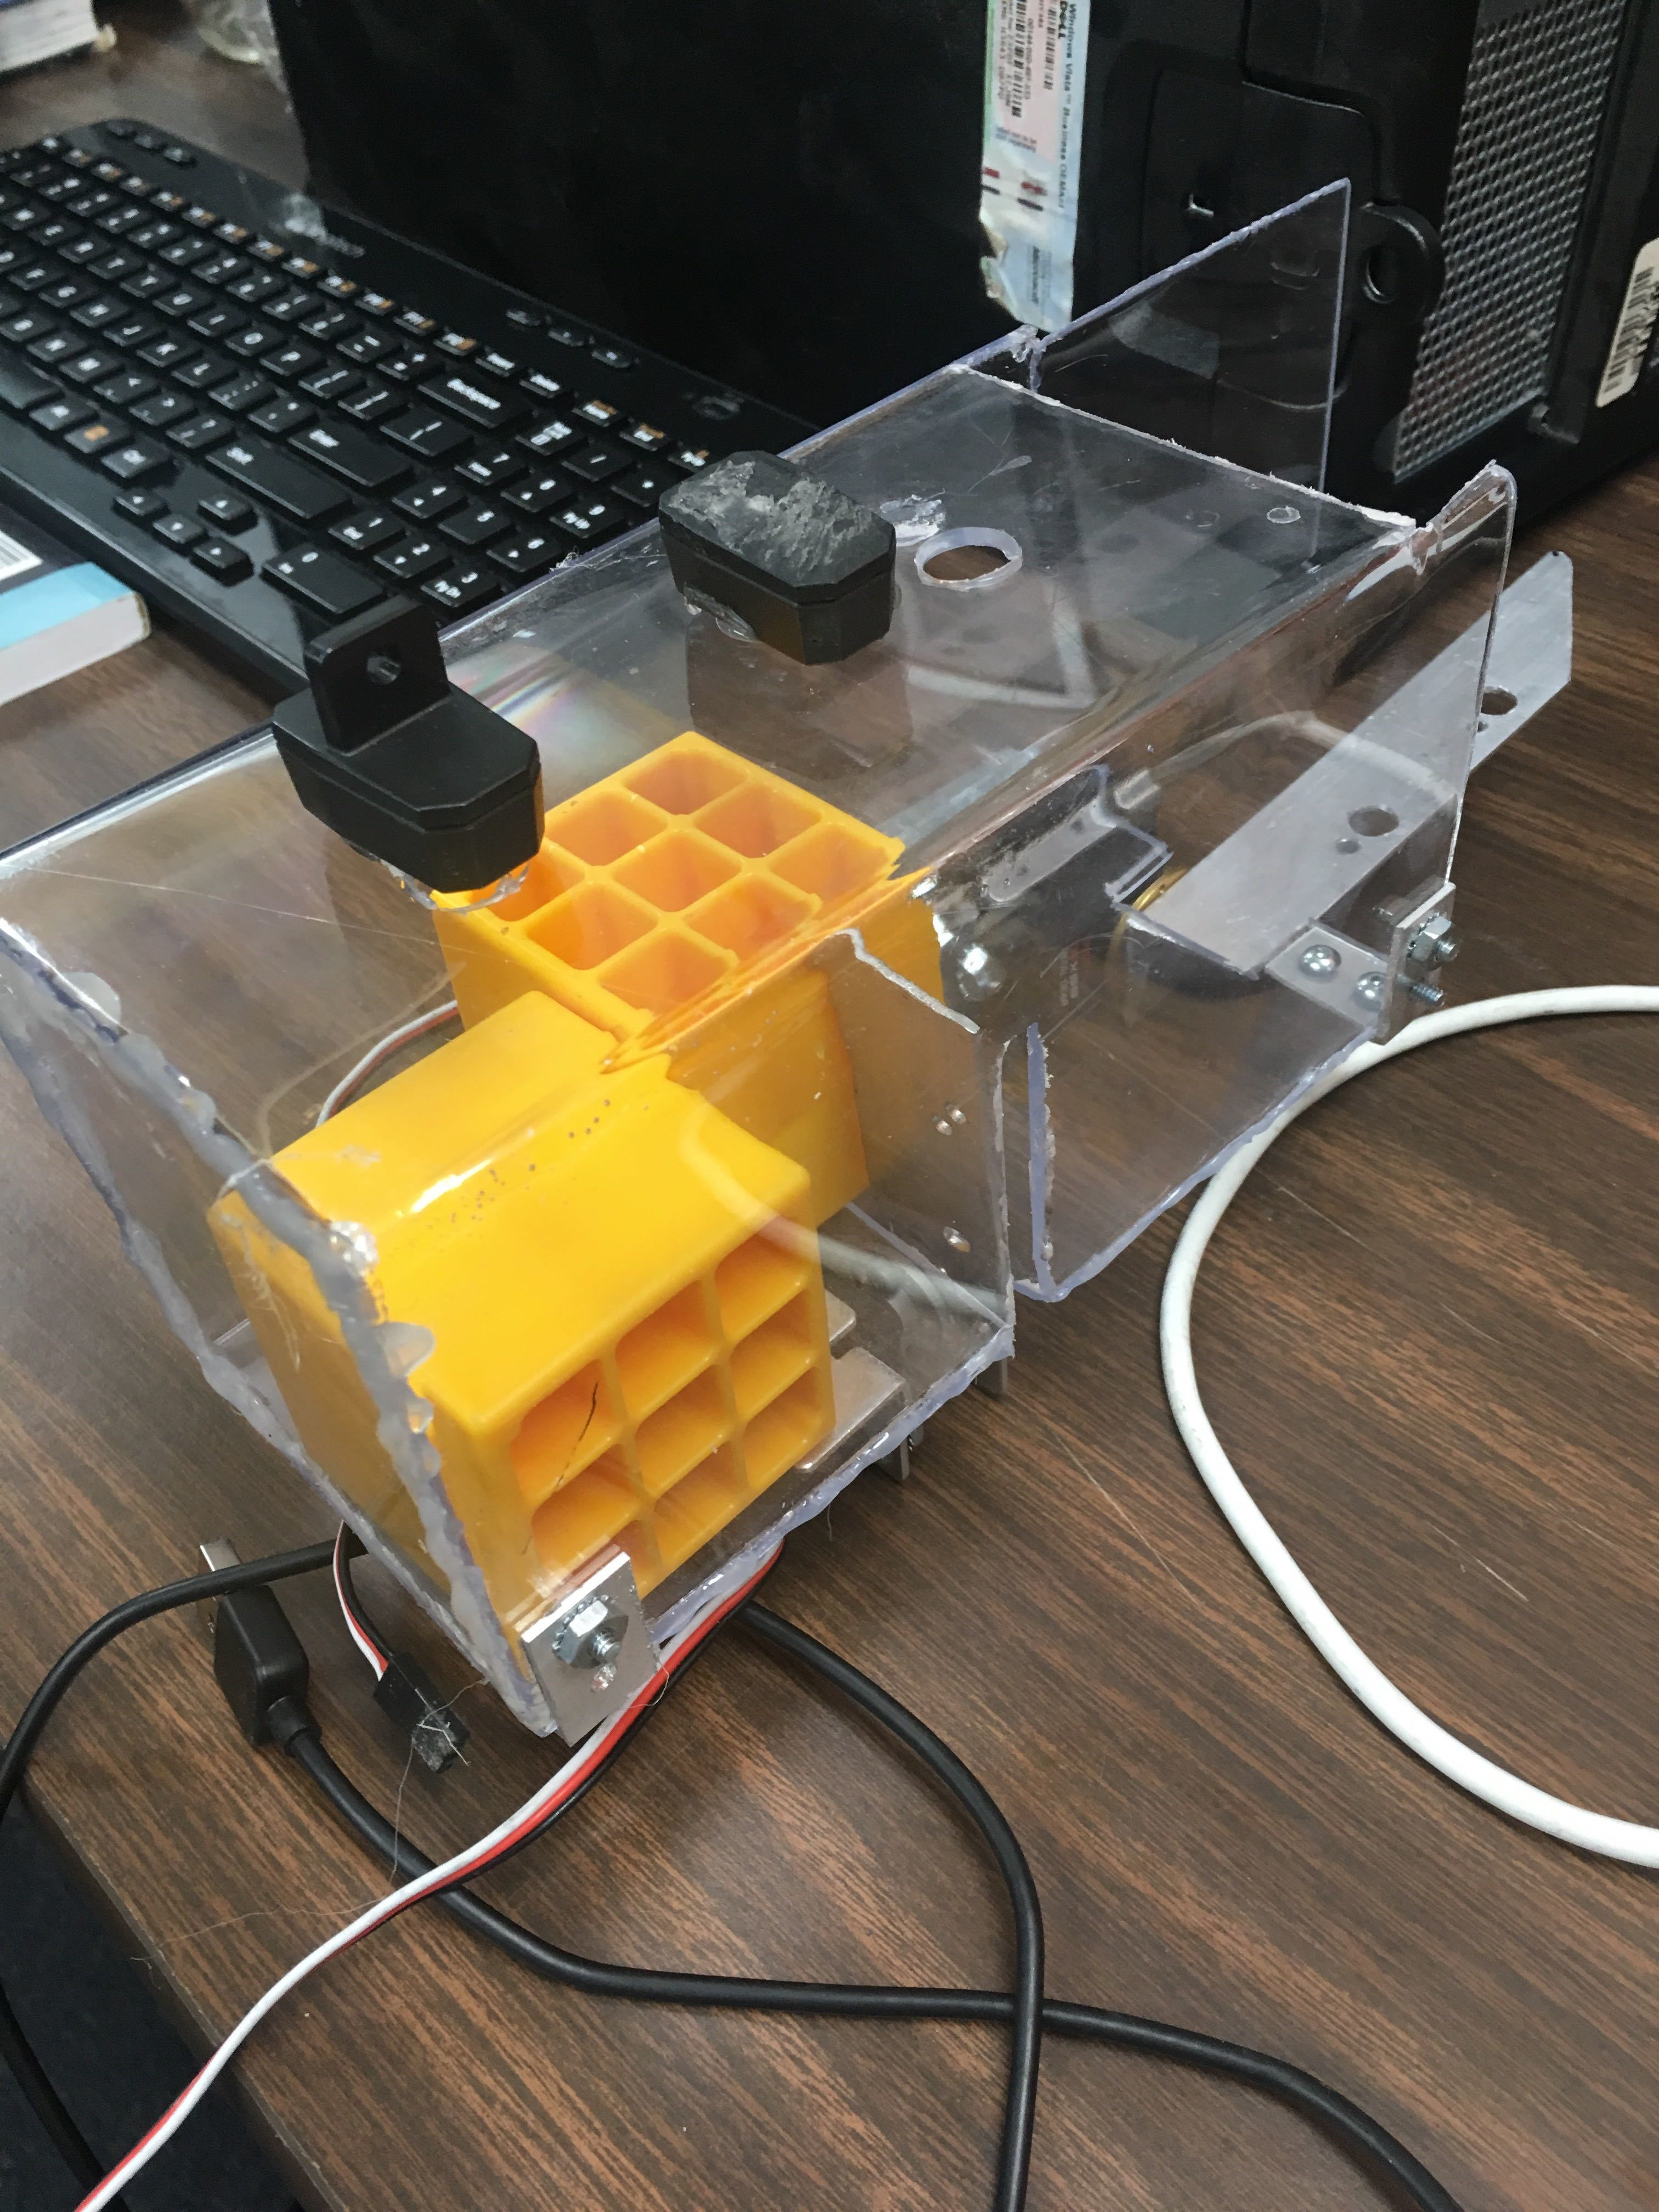
\includegraphics[width=.6 \textwidth]{14_12-03/images/cartridge1.JPG}
    \caption{Cartridge prototype}
    \label{fig:cartridge}
\end{figure}

\begin{figure}
    \centering
    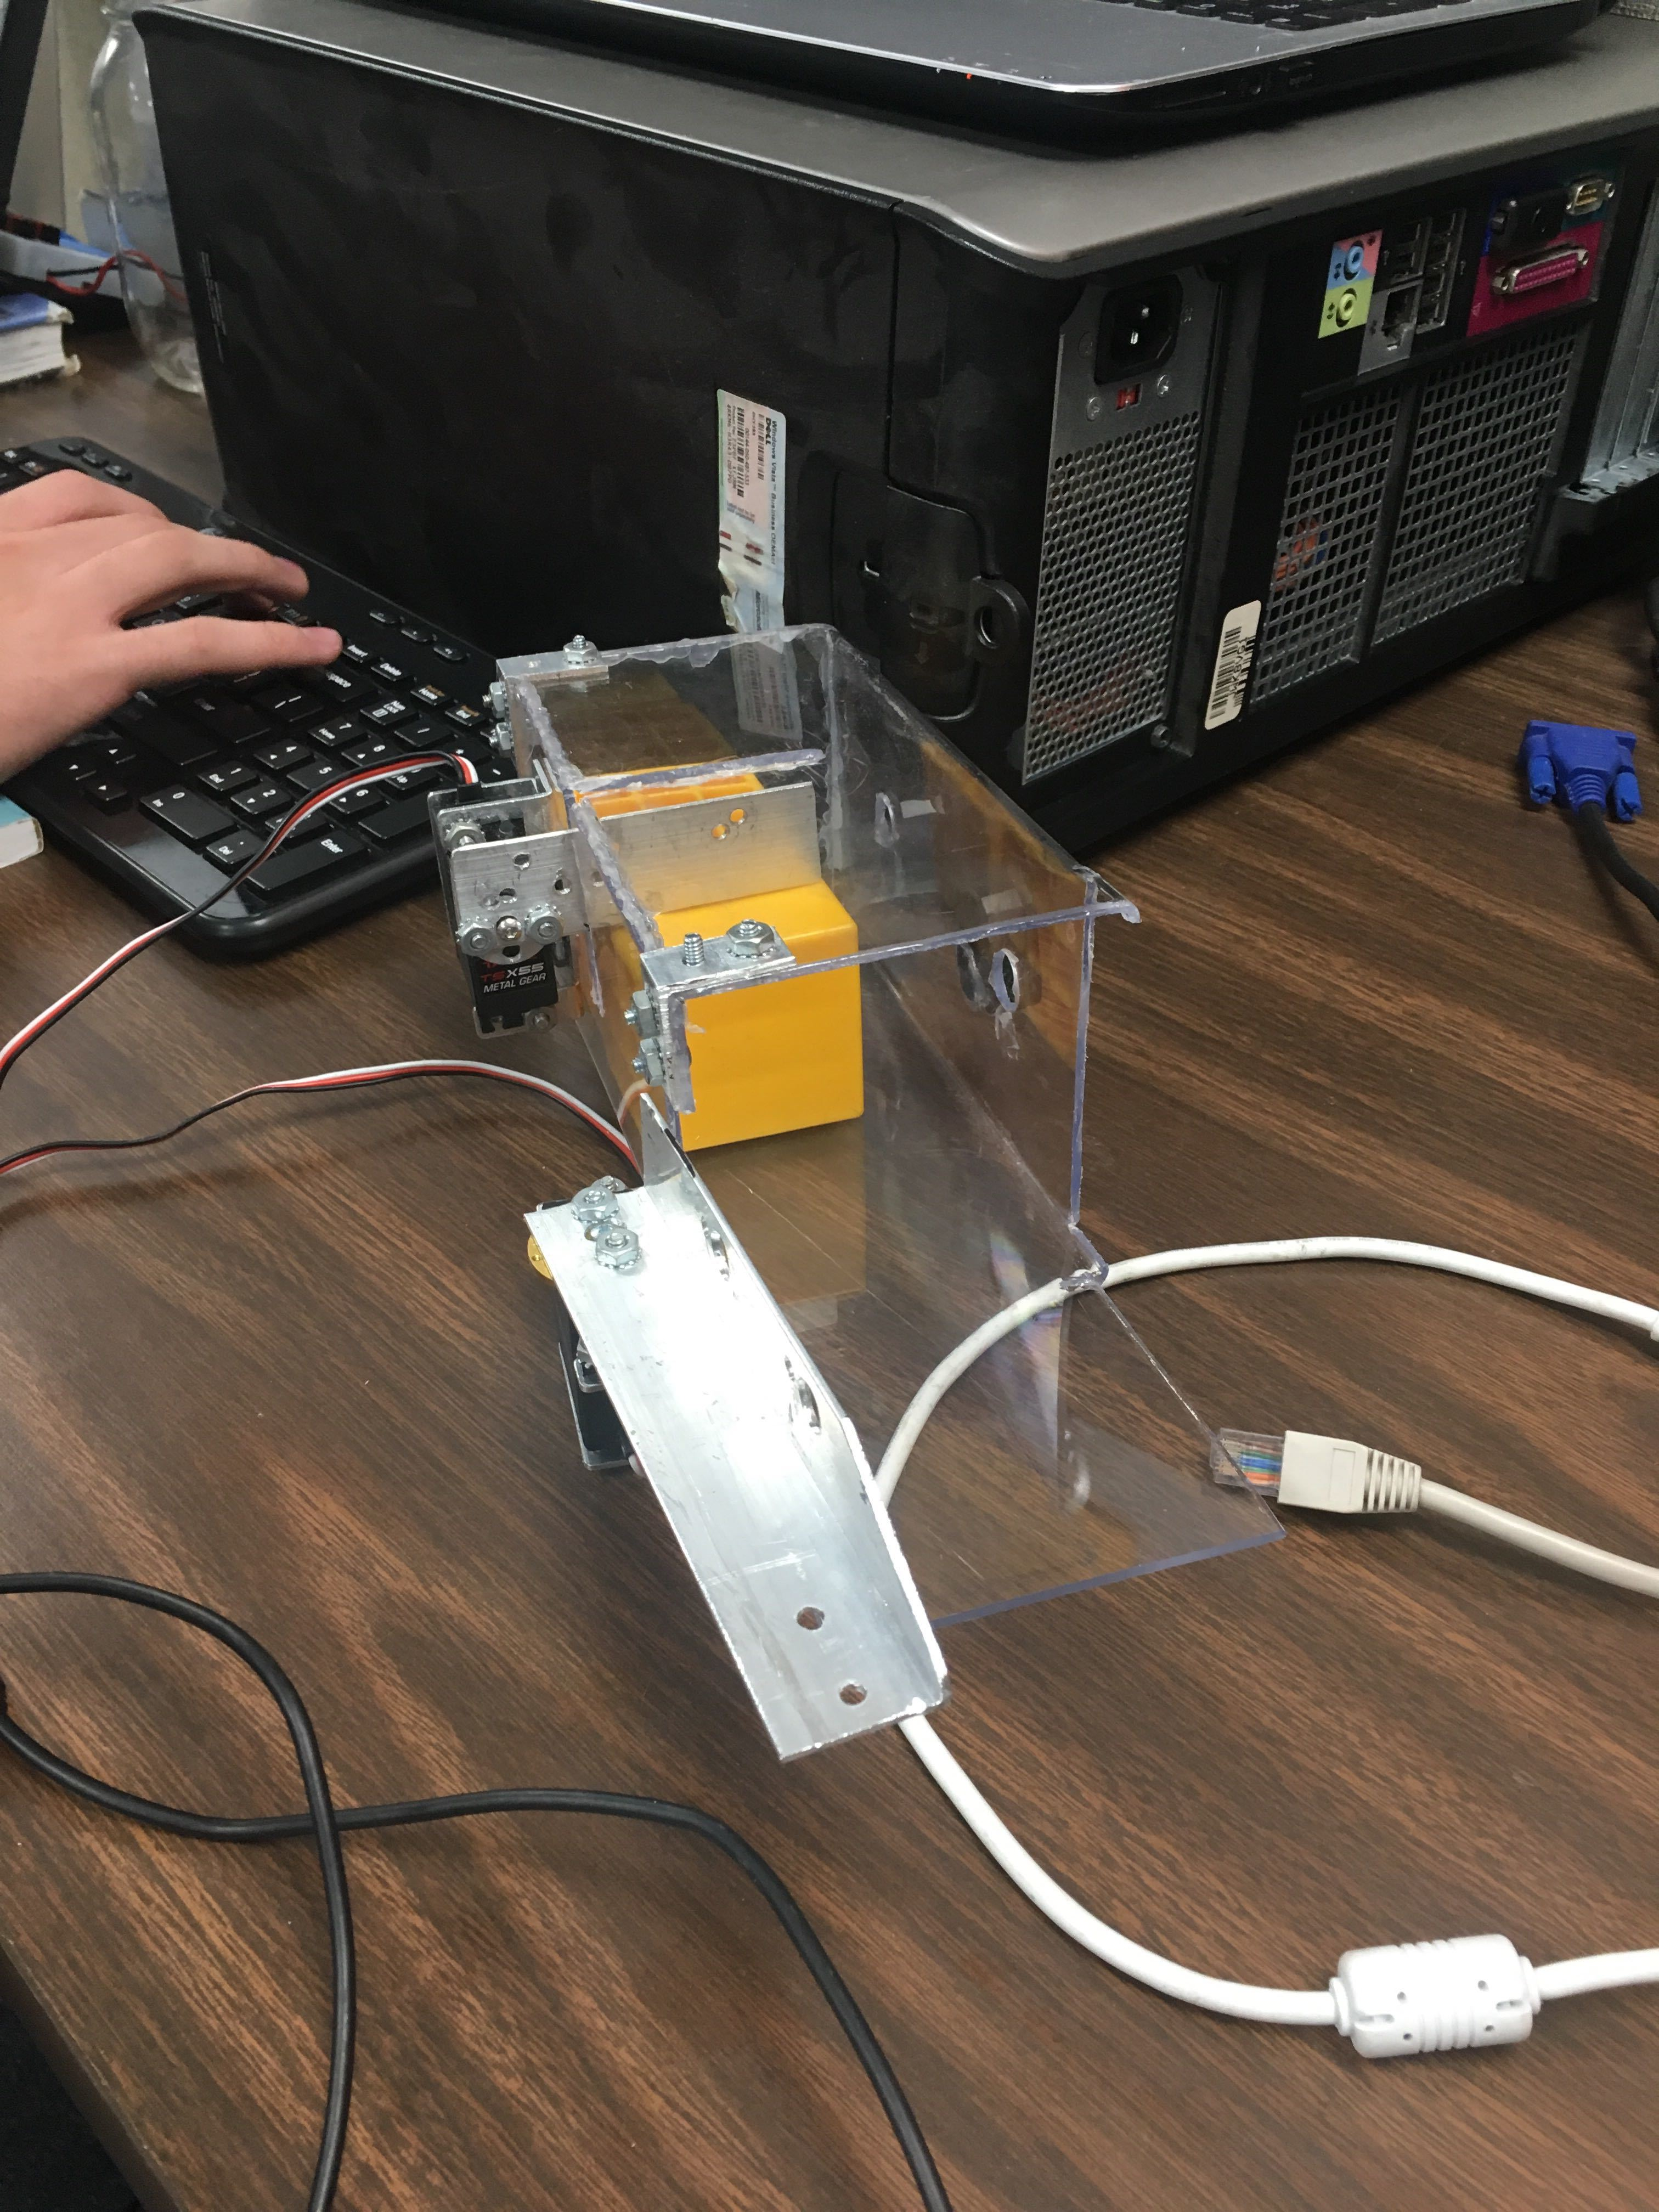
\includegraphics[width=.6 \textwidth]{14_12-03/images/cartridge3.JPG}
    \caption{Cartridge prototype}
    \label{fig:thing}
\end{figure}

\subsection{Latching Hook}
%! CADing and doing math for the hook.
After Ben and Shawn prototyped the servo and pin latch mechanism, the team realized that a simpler design would be easier to control and manufacture. Ben started CADing the part and Kelly suggested they use math to find how thick they should make the aluminum. So Kelly, Ben, and Aidan started discussing it, they used a combination of physics and trigonometry to determine the stress as shown in figure \ref{fig:math} . Then they used the stress analysis tool in Inventor to see where the most stress was and were the aluminum would, in theory, bend or break as shown in fig \ref{fig:stress}. They found that the red was only around 1.5 ksi, so they looked up the max ksi before elastic deformation and found that it was around 40 ksi. So the aluminum was perfectly fine.


\subsection{Drive-Train Update}
%! Re-CADing the Drive-Train.
After a rush finish for the drive-train, due to the Burlingame tournament. The team felt it was necessary to simplify the drive-train to allow for more room and more precise mounting of other mechanism to the drive base. Currently on the robot their is a separate aluminum plate that holds the intake to the drive-train, which is structurally  weak and allows for a lot of excess vibrations when the intake is running. As a result it was re-CADed so that the added on part was cut out with the inside plate as a whole this allows for more room between each drive half, along with being more structurally sound. Another very important change is the placement of the rear cross brace closest to the linear lift. It was moved closer to the motors to allow for more room, so that the lift motor and spool can be mounted directly under the lift for the pull down string. 

\begin{figure}
    \centering
    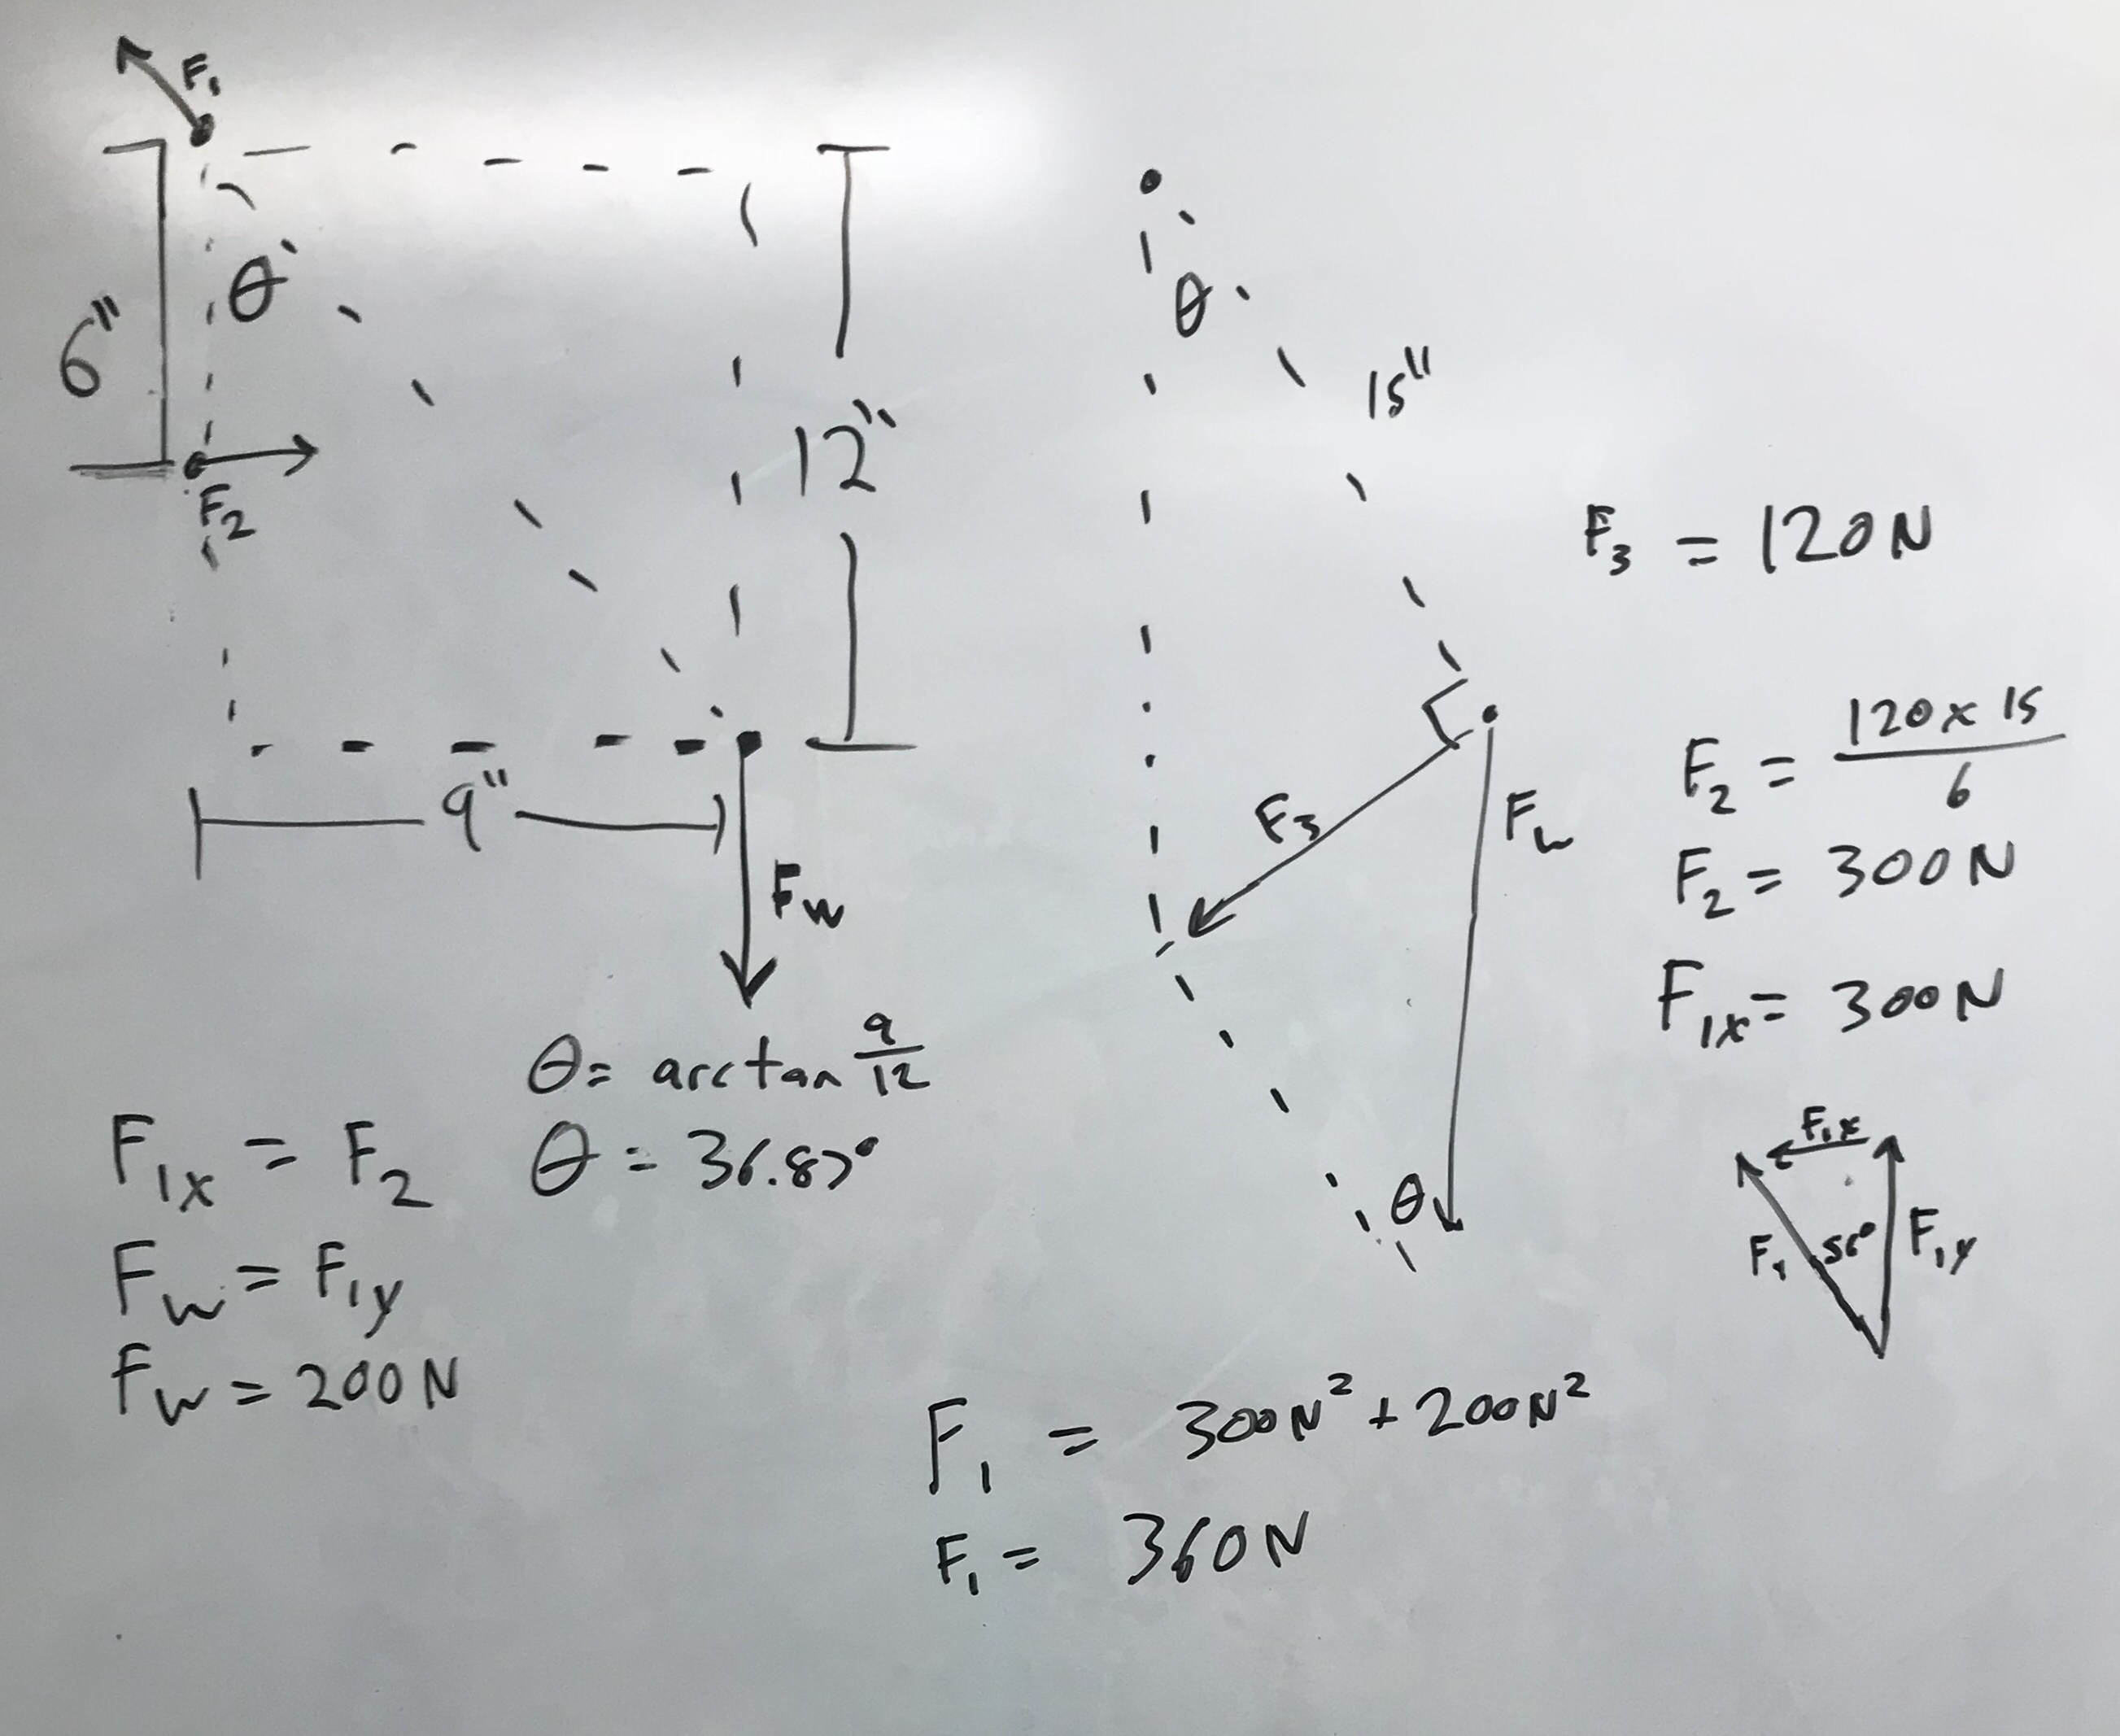
\includegraphics[width=.6 \textwidth]{14_12-03/images/Math.jpg}
    \caption{Stress Math}
    \label{fig:math}
\end{figure}

\begin{figure}
    \centering
    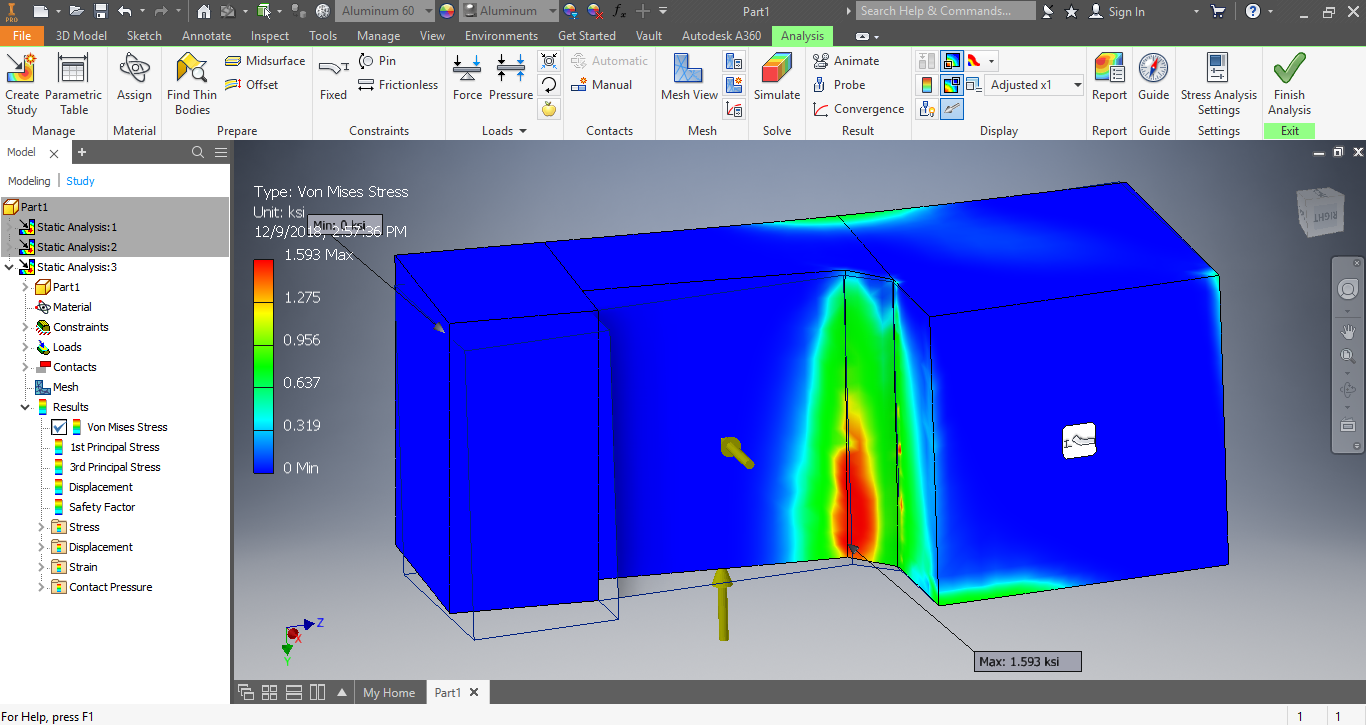
\includegraphics[width=.6\textwidth]{14_12-03/images/Stress_Analysis.png}
    \caption{Stress Analysis}
    \label{fig:stress}
\end{figure}
\end{document}
